\chapter{Vector Calculus: Green, Stokes, and Divergence}

\providecommand{\oiint}{\oint\kern-0.62em\oint}

Every theorem in this chapter is secretly the same theorem. You already know it.
Back in Chapter~21 the Fundamental Theorem of Calculus told you that to add up a
rate of change over an interval, you do not have to actually add anything up --
you just look at the two endpoints:
\[
  \int_a^b F'(x)\,\dd x \;=\; F(b) - F(a).
\]
The whole interior of $[a,b]$ -- the infinitely many places where $F$ is wiggling
and changing -- collapses into two numbers at the boundary. The accumulated change
inside is remembered entirely by the edge.

That sentence -- \emph{the boundary remembers the inside} -- is the soul of
vector calculus. The great theorems of this chapter (Green's theorem, the
divergence theorem, Stokes' theorem) all say the same thing in higher dimensions:
to learn what is happening throughout a region, you only have to walk around its
\emph{boundary}. An integral over a solid blob equals an integral over the skin
that wraps it. An integral over a flat patch equals an integral around the loop
that fences it. In each case a $d$-dimensional accumulation is paid off by a
$(d{-}1)$-dimensional reckoning at the edge. The Fundamental Theorem of Calculus
was the one-dimensional baby version, where the ``boundary'' of an interval is
just its two endpoints.

To say all this we need a new main character: the \emph{vector field}. So far our
functions have eaten points and spat out numbers. Now they will spit out
\emph{arrows} -- a velocity at every point of a flowing river, a force at every
point in a magnetic field, a push at every point of the wind. Once we can
integrate arrows along curves and across surfaces, the great theorems write
themselves.

\begin{focusbox}
One idea, four faces:
\[
\begin{aligned}
\text{FTC:} &\quad \int_a^b F' = F(b)-F(a) &&\text{(1D: endpoints)}\\
\text{Gradient theorem:} &\quad \int_C \grad f\cdot \dd\vec r = f(\text{end})-f(\text{start}) &&\text{(curve: endpoints)}\\
\text{Green / Stokes:} &\quad \iint_S (\text{curl}) = \oint_{\partial S}(\text{field}) &&\text{(patch: boundary loop)}\\
\text{Divergence:} &\quad \iiint_V (\text{div}) = \oiint_{\partial V}(\text{flux}) &&\text{(solid: boundary skin)}
\end{aligned}
\]
Read every line as: \emph{accumulate a derivative inside} $=$ \emph{read the
field on the boundary}.
\end{focusbox}

\chapterline

\section{Vector fields: a function that grows arrows}
\label{ch35:fields}

A \emph{scalar field} assigns a number to each point: temperature in a room,
altitude on a map, pressure in the ocean. We have been studying these for two
chapters under the name $f(x,y)$ or $f(x,y,z)$. A \emph{vector field} assigns an
\emph{arrow} -- a vector -- to each point instead.

\begin{definition}[Vector field]
\label{ch35:def-field}
A vector field on a region of the plane is a function
\[
  \vec F(x,y) = \big(P(x,y),\, Q(x,y)\big) = P(x,y)\,\vec i + Q(x,y)\,\vec j,
\]
that assigns to each point $(x,y)$ the vector $\vec F(x,y)$. In three dimensions,
$\vec F(x,y,z) = (P,Q,R)$, with three component functions. We draw it by planting
the arrow $\vec F(x,y)$ with its \emph{tail} at the point $(x,y)$.
\end{definition}

The picture is everything. Below is the field $\vec F(x,y) = (-y, x)$. At each
point we draw the arrow $(-y,x)$. Notice it always points ninety degrees
counterclockwise from the position vector $(x,y)$ -- so the whole field swirls
around the origin like water circling a drain, or a spinning turntable.

\begin{figure}[H]
\centering
\begin{tikzpicture}[scale=1.15,>={Stealth[length=4pt]}]
\draw[->,gray!55] (-2.5,0)--(2.5,0) node[right]{\scriptsize $x$};
\draw[->,gray!55] (0,-2.5)--(0,2.5) node[above]{\scriptsize $y$};
\foreach \x in {-2,-1,0,1,2}{
  \foreach \y in {-2,-1,0,1,2}{
    \draw[->,blue!55!black] (\x,\y) -- ++({-\y*0.28},{\x*0.28});
  }
}
\end{tikzpicture}
\caption{The rotational field $\vec F(x,y)=(-y,x)$. Every arrow is perpendicular
to the line joining it to the origin, so the field circulates counterclockwise.
This is the canonical ``swirl,'' and it will be our running example for curl.}
\label{ch35:fig-swirl}
\end{figure}

Here is a second essential example: a \emph{source} field
$\vec F(x,y) = (x,y)$, where every arrow points radially \emph{outward}, away
from the origin, growing longer as you move out. Think of it as the velocity of
gas billowing out of a vent at the origin.

\begin{figure}[H]
\centering
\begin{tikzpicture}[scale=1.15,>={Stealth[length=4pt]}]
\draw[->,gray!55] (-2.5,0)--(2.5,0) node[right]{\scriptsize $x$};
\draw[->,gray!55] (0,-2.5)--(0,2.5) node[above]{\scriptsize $y$};
\foreach \x in {-2,-1,0,1,2}{
  \foreach \y in {-2,-1,0,1,2}{
    \draw[->,red!60!black] (\x,\y) -- ++({\x*0.24},{\y*0.24});
  }
}
\end{tikzpicture}
\caption{The source field $\vec F(x,y)=(x,y)$: arrows point straight out from the
origin and grow with distance. This is the canonical ``spreading'' field, and it
will be our running example for divergence.}
\label{ch35:fig-source}
\end{figure}

\begin{intuitionbox}
Two motions live inside every vector field, and the rest of the chapter is about
measuring them. \textbf{Circulation}: does the field tend to \emph{spin} you
around a loop? (The swirl in Figure~\ref{ch35:fig-swirl} does.) \textbf{Flux}:
does the field tend to \emph{carry stuff out through} a boundary? (The source in
Figure~\ref{ch35:fig-source} does.) Curl will measure local spin; divergence
will measure local spreading. Everything else is bookkeeping.
\end{intuitionbox}

\begin{applicationbox}
Vector fields are how physics stores the state of the invisible. The wind on a
weather map is $\vec F(x,y)=$ (velocity of air). The gravitational pull near a
planet is a field of arrows pointing inward. The electric field around a charge,
the magnetic field around a wire, the flow of heat through a wall, the current in
the ocean -- each is a vector field, and each obeys laws written in the language
of this chapter. Maxwell's four equations of electromagnetism are \emph{nothing
but} statements about the divergence and curl of two vector fields.
\end{applicationbox}

\section{Line integrals: adding a field along a path}
\label{ch35:lineint}

\subsection{Work, and why we multiply force by displacement}

Drag a box across a floor. The work you do is force times distance -- but only the
\emph{part of the force that lies along the motion} counts. Push straight down on
a box and slide it sideways and you have done no work on it at all; your downward
force is perpendicular to the sideways motion. The honest measure of work for a
constant force $\vec F$ over a straight displacement $\vec d$ is the dot product
\[
  W = \vec F \cdot \vec d = \abs{\vec F}\,\abs{\vec d}\cos\theta,
\]
which keeps exactly the component of $\vec F$ pointing along $\vec d$ and throws
away the perpendicular part.

Now let the force vary from point to point -- a vector field $\vec F$ -- and let
the path curve. We do what we always do in calculus: chop the path into tiny
nearly-straight pieces, on each piece treat the force as roughly constant, compute
the little bit of work $\vec F\cdot\Delta\vec r$, add them all up, and take the
limit as the pieces shrink. That limit is the \emph{line integral}.

\begin{definition}[Line integral of a vector field]
\label{ch35:def-lineint}
Let $C$ be a curve traced by $\vec r(t)=(x(t),y(t))$ for $t\in[a,b]$, and let
$\vec F$ be a vector field along it. The line integral of $\vec F$ along $C$ is
\[
  \int_C \vec F\cdot \dd\vec r
  \;=\; \int_a^b \vec F\big(\vec r(t)\big)\cdot \vec r\,'(t)\,\dd t.
\]
Writing $\vec F=(P,Q)$ and $\dd\vec r = (\dd x,\dd y)$, this is also written
$\displaystyle \int_C P\,\dd x + Q\,\dd y$.
\end{definition}

\begin{whybox}
Why does $\dd\vec r$ become $\vec r\,'(t)\,\dd t$? Because $\vec r\,'(t)$ is the
velocity vector -- it points along the curve and its length is the speed. Over a
tiny time $\dd t$ the path advances by the little displacement vector
$\dd\vec r = \vec r\,'(t)\,\dd t$. Dotting the force against this displacement
gives the infinitesimal work $\vec F\cdot\dd\vec r$, and integrating in $t$ adds
them along the curve. The parameter $t$ is just a clock we run along the path; the
answer, reassuringly, will not depend on \emph{how fast} we run it.
\end{whybox}

\begin{walkbox}
Why doesn't the speed of traversal change the answer? If you re-parametrize and
move twice as fast, then $\vec r\,'$ doubles but the time interval $\dd t$ halves,
and the product $\vec r\,'(t)\,\dd t = \dd\vec r$ is unchanged -- it is a geometric
displacement, blind to the clock. (Reversing direction, however, flips every
$\dd\vec r$, so it flips the sign of the integral. Orientation matters; speed does
not.)
\end{walkbox}

\subsection{A worked line integral, step by step}

\begin{example}[Work along a parabola]
\label{ch35:ex-parab}
Compute $\displaystyle\int_C \vec F\cdot\dd\vec r$ for $\vec F(x,y)=(y,\,x^2)$
along the parabola $y=x^2$ from $(0,0)$ to $(2,4)$.

\textbf{Step 1 -- parametrize.} Let $x=t$, $y=t^2$, so $\vec r(t)=(t,t^2)$ for
$t\in[0,2]$. Then $\vec r\,'(t)=(1,2t)$.

\textbf{Step 2 -- evaluate the field on the path.}
$\vec F(\vec r(t)) = (y,\,x^2)\big|_{x=t,\,y=t^2} = (t^2,\, t^2)$.

\textbf{Step 3 -- dot.}
$\vec F(\vec r(t))\cdot\vec r\,'(t) = (t^2)(1)+(t^2)(2t) = t^2 + 2t^3.$

\textbf{Step 4 -- integrate.}
\[
  \int_0^2 (t^2 + 2t^3)\,\dd t
  = \left[\frac{t^3}{3} + \frac{t^4}{2}\right]_0^2
  = \frac{8}{3} + 8 = \frac{32}{3}.
\]
The total work is $\tfrac{32}{3}$. The recipe never changes: parametrize, plug in,
dot, integrate a single ordinary integral in $t$.
\end{example}

\begin{figure}[H]
\centering
\begin{tikzpicture}[scale=1.0,>={Stealth[length=4pt]}]
\begin{axis}[
  width=8.4cm, height=6.4cm,
  axis lines=middle, xlabel={\scriptsize $x$}, ylabel={\scriptsize $y$},
  xmin=-0.4, xmax=2.6, ymin=-0.4, ymax=4.6,
  xtick={1,2}, ytick={1,2,3,4}, tick label style={font=\scriptsize},
  clip=false,
]
% the path y = x^2
\addplot[curveblue, very thick, domain=0:2, samples=80] {x^2};
\node[curveblue, anchor=west] at (axis cs:1.55,2.5) {\scriptsize $C:\ y=x^2$};
% field arrows F=(y,x^2)=(t^2,t^2) at sample points (t,t^2) along the path
\addplot[tangentred, ->, quiver={u=\thisrow{u}, v=\thisrow{v}}, only marks, mark=none]
  table[row sep=\\]{
    x    y    u     v    \\
    0.5  0.25 0.075 0.075 \\
    1.0  1.0  0.30  0.30  \\
    1.5  2.25 0.675 0.675 \\
    2.0  4.0  1.20  1.20  \\
  };
% endpoints
\addplot[only marks, mark=*, mark size=1.4pt, black] coordinates {(0,0) (2,4)};
\node[anchor=north west] at (axis cs:0.05,-0.05) {\scriptsize $(0,0)$};
\node[anchor=west] at (axis cs:2.05,4) {\scriptsize $(2,4)$};
\end{axis}
\end{tikzpicture}
\caption{The work integral of Example~\ref{ch35:ex-parab}: we walk the parabola
$C$ (blue) from $(0,0)$ to $(2,4)$. The line integral adds up, at each point of the
path, the component of the field $\vec F=(y,x^2)$ that lies along the blue curve.
The along-path total works out to $\tfrac{32}{3}$.}
\label{ch35:fig-work}
\end{figure}

\begin{trapbox}
A line integral $\int_C \vec F\cdot\dd\vec r$ is \emph{not} the same as the
arc-length integral $\int_C f\,\dd s$ you may have seen (mass of a wire). The dot
product version measures the field's component \emph{along} the curve and is
sensitive to direction; reversing the path negates it. The arc-length version uses
$\dd s = \abs{\vec r\,'(t)}\,\dd t$ (a length, always positive) and does not care
about direction. They answer different questions. This chapter is almost entirely
about the dot-product kind.
\end{trapbox}

\section{Conservative fields: when the path does not matter}
\label{ch35:conservative}

In Example~\ref{ch35:ex-parab} the answer depended on the curve we chose. For some
special fields it does \emph{not}: the work depends only on where you start and
where you stop, never on the route between. These are the \emph{conservative}
fields, and they are exactly the fields that are gradients.

\begin{theorem}[Fundamental Theorem for line integrals / Gradient theorem]
\label{ch35:thm-gradient}
If $\vec F = \grad f$ for some scalar function $f$ (a \emph{potential}), then for
any curve $C$ from point $A$ to point $B$,
\[
  \int_C \grad f\cdot \dd\vec r = f(B) - f(A).
\]
The integral depends only on the endpoints. In particular, around any closed loop
($A=B$), $\displaystyle\oint_C \grad f\cdot\dd\vec r = 0$.
\end{theorem}

\begin{whybox}
This is the Fundamental Theorem of Calculus wearing a coat. Parametrize $C$ by
$\vec r(t)$, $t\in[a,b]$, and watch the chain rule do the entire job:
\[
  \int_C \grad f\cdot\dd\vec r
  = \int_a^b \grad f(\vec r(t))\cdot \vec r\,'(t)\,\dd t
  = \int_a^b \frac{\dd}{\dd t}\Big[f(\vec r(t))\Big]\,\dd t
  = f(\vec r(b)) - f(\vec r(a)).
\]
The middle equality is the multivariable chain rule (Chapter~33):
$\grad f\cdot\vec r\,' = \dv{}{t}f(\vec r(t))$. So the integrand was a perfect
derivative all along, and the ordinary FTC finishes it. ``The boundary remembers
the inside'' here means: the two endpoints remember the whole accumulated climb.
\end{whybox}

\begin{intuitionbox}
A potential $f$ is an \emph{altitude}. The field $\grad f$ points straight uphill,
and its work is the height you gain. Walk any trail from the trailhead to the
summit -- switchbacks, scenic detours, whatever -- and the elevation gained is the
same, because it is just (summit altitude) minus (trailhead altitude). Walk a loop
back to where you started and you gain zero net altitude. That is the whole content
of conservativeness. A field is conservative precisely when it has an altitude
function.
\end{intuitionbox}

\begin{figure}[H]
\centering
\begin{tikzpicture}[scale=1.0,>={Stealth[length=4pt]}]
\begin{axis}[
  width=8.6cm, height=6.6cm,
  axis lines=middle, xlabel={\scriptsize $x$}, ylabel={\scriptsize $y$},
  xmin=-2.3, xmax=2.3, ymin=-2.3, ymax=2.3,
  xtick=\empty, ytick=\empty,
]
% level curves of the potential f = x^2 + y^2 (circles)
\addplot[gray!60, samples=90, domain=0:360] ({0.7*cos(x)},{0.7*sin(x)});
\addplot[gray!60, samples=90, domain=0:360] ({1.3*cos(x)},{1.3*sin(x)});
\addplot[gray!60, samples=90, domain=0:360] ({1.9*cos(x)},{1.9*sin(x)});
% gradient arrows F = grad f = (2x,2y), scaled, pointing outward
\addplot[targetgreen, ->, quiver={u=\thisrow{u}, v=\thisrow{v}}, only marks, mark=none]
  table[row sep=\\]{
    x     y     u      v     \\
    -1.5  -1.5  -0.42  -0.42 \\
    -0.8  -1.5  -0.224 -0.42 \\
     0.8  -1.5   0.224 -0.42 \\
     1.5  -1.5   0.42  -0.42 \\
    -1.5  -0.8  -0.42  -0.224 \\
    -0.8  -0.8  -0.224 -0.224 \\
     0.8  -0.8   0.224 -0.224 \\
     1.5  -0.8   0.42  -0.224 \\
    -1.5   0.8  -0.42   0.224 \\
    -0.8   0.8  -0.224  0.224 \\
     0.8   0.8   0.224  0.224 \\
     1.5   0.8   0.42   0.224 \\
    -1.5   1.5  -0.42   0.42 \\
    -0.8   1.5  -0.224  0.42 \\
     0.8   1.5   0.224  0.42 \\
     1.5   1.5   0.42   0.42 \\
  };
\node[gray!50!black, anchor=west] at (axis cs:0.95,1.7) {\scriptsize level sets of $f$};
\node[targetgreen!60!black, anchor=west] at (axis cs:1.0,-2.0) {\scriptsize $\grad f$};
\end{axis}
\end{tikzpicture}
\caption{A conservative field is a gradient. Here $f(x,y)=x^2+y^2$ is the
``altitude.'' Its level sets (gray circles) are the contour lines, and the field
$\grad f=(2x,2y)$ (green arrows) crosses them at right angles, always pointing
uphill. Work done along any path is just the change in altitude between its
endpoints; around a closed loop it is zero.}
\label{ch35:fig-gradient}
\end{figure}

\subsection{How to test for, and find, a potential}

In the plane, write $\vec F=(P,Q)$. If $\vec F=\grad f=(f_x,f_y)$ then
$P=f_x$ and $Q=f_y$. By Clairaut's theorem (mixed partials commute, Chapter~32),
\[
  \pdv{P}{y} = f_{xy} = f_{yx} = \pdv{Q}{x}.
\]
So a \emph{necessary} condition is $P_y = Q_x$. On a region with no holes (a
``simply connected'' region -- one where every loop can be shrunk to a point) this
condition is also \emph{sufficient}: it guarantees a potential exists.

\begin{example}[Finding a potential]
\label{ch35:ex-potential}
Is $\vec F=(2xy + 3,\; x^2 - 1)$ conservative? Here $P=2xy+3$, $Q=x^2-1$.

\textbf{Test.} $P_y = 2x$ and $Q_x = 2x$. They agree, and the plane has no holes,
so a potential exists.

\textbf{Build it.} We need $f$ with $f_x = 2xy+3$. Integrate in $x$ (treating $y$
as constant):
\[
  f(x,y) = x^2 y + 3x + g(y),
\]
where the ``constant'' of integration is allowed to depend on $y$. Now demand
$f_y = Q$:
\[
  f_y = x^2 + g'(y) \overset{!}{=} x^2 - 1 \;\Rightarrow\; g'(y) = -1 \;\Rightarrow\; g(y) = -y + C.
\]
So $f(x,y) = x^2y + 3x - y + C$. As a check, $\grad f = (2xy+3,\; x^2-1)=\vec F$.
Now any line integral of $\vec F$ is trivial: from $(0,0)$ to $(1,2)$ it is
$f(1,2)-f(0,0) = (2 + 3 - 2) - 0 = 3$, no matter the path.
\end{example}

\begin{trapbox}
The hole matters. The famous swirl
$\vec F = \big(\frac{-y}{x^2+y^2}, \frac{x}{x^2+y^2}\big)$ satisfies $P_y=Q_x$
\emph{everywhere it is defined}, yet $\oint \vec F\cdot\dd\vec r = 2\pi \ne 0$
around the unit circle. It is \emph{not} conservative. The catch: it is undefined
at the origin, so its domain has a hole, and the loop around that hole cannot be
shrunk to a point. The test $P_y=Q_x$ only promises a potential on a
\emph{simply connected} domain. Topology sneaks into calculus right here.
\end{trapbox}

\begin{historybox}
The word ``conservative'' comes from physics, not bookkeeping. If $\vec F$ is a
force with potential energy $U$ (so $\vec F=-\grad U$), then the work done equals
the drop in $U$, and the quantity (kinetic $+$ potential energy) stays constant
along any motion -- energy is \emph{conserved}. Gravity and electrostatics are
conservative; friction is not (it bleeds energy as heat, and its loop integral is
nonzero -- that is why perpetual-motion machines fail). The nineteenth-century
drive to understand which forces conserve energy, led by Helmholtz and Kelvin, is
exactly what forced mathematicians to clarify when a field is a gradient.
\end{historybox}

\section{Green's theorem: the first ``boundary remembers inside''}
\label{ch35:green}

We now meet the first of the three great theorems, and the one easiest to picture.
Green's theorem relates a line integral \emph{around} a closed loop $C$ to a double
integral \emph{over} the flat region $D$ that the loop encloses.

\begin{theorem}[Green's theorem, circulation form]
\label{ch35:thm-green}
Let $D$ be a region in the plane bounded by a simple closed curve $C$, traversed
counterclockwise. If $\vec F=(P,Q)$ has continuous partials on $D$, then
\[
  \oint_C P\,\dd x + Q\,\dd y \;=\; \iint_D \left(\pdv{Q}{x} - \pdv{P}{y}\right)\dd A.
\]
\end{theorem}

The quantity $\pdv{Q}{x}-\pdv{P}{y}$ is the \emph{microscopic circulation} -- the
``curl'' of the field, which we meet properly in the next section. Green's theorem
says: the total swirl around the boundary equals the sum of all the little swirls
inside.

\begin{happeningbox}
Here is the real mechanism, and it is beautiful. Tile the region $D$ with tiny
rectangles. For each tiny rectangle, run the line integral around its own little
boundary, counterclockwise. Now add up all these little loop integrals. Look at
any internal edge shared by two adjacent tiles: one tile traverses it
left-to-right, its neighbor traverses the \emph{same} edge right-to-left. The two
contributions are equal and opposite -- they \textbf{cancel}. Every interior edge
cancels against its neighbor. The \emph{only} edges that survive the great
cancellation are the ones on the outer boundary of $D$, where there is no neighbor
to cancel with. So
\[
  \sum_{\text{tiles}} (\text{tiny loop integral}) = (\text{big boundary integral}).
\]
Meanwhile each tiny loop integral, by a short computation, equals
$\big(Q_x - P_y\big)\times(\text{area of tile})$. Summing those is the double
integral. The interior cancellation is \emph{exactly} the same telescoping that
made the Fundamental Theorem of Calculus work, where the inner endpoints of
adjacent subintervals cancelled and only $a$ and $b$ survived.
\end{happeningbox}

\begin{figure}[H]
\centering
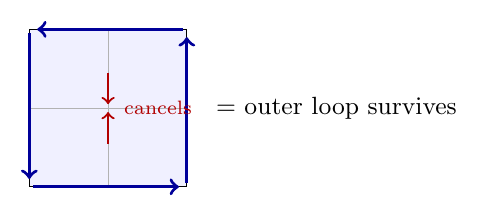
\begin{tikzpicture}[scale=1.0]
% region tiled into 4 squares, showing internal-edge cancellation
\draw[fill=blue!6] (0,0) rectangle (2,2);
\draw[gray!60] (1,0)--(1,2);
\draw[gray!60] (0,1)--(2,1);
% outer boundary CCW arrows
\draw[->,blue!60!black,very thick] (0.05,0) -- (1.9,0);
\draw[->,blue!60!black,very thick] (2,0.05) -- (2,1.9);
\draw[->,blue!60!black,very thick] (1.95,2) -- (0.1,2);
\draw[->,blue!60!black,very thick] (0,1.95) -- (0,0.1);
% internal shared edge: two opposing arrows that cancel
\draw[->,red!70!black,thick] (1,0.55) -- (1,0.95);
\draw[->,red!70!black,thick] (1,1.45) -- (1,1.05);
\node[red!70!black,right] at (1.08,1.0) {\scriptsize cancels};
\node at (3.9,1) {\small $=$ outer loop survives};
\end{tikzpicture}
\caption{Green's theorem by cancellation. Sum the counterclockwise loop integrals
of all small tiles. On every shared internal edge the two neighbors run opposite
ways and cancel (red). Only the outer boundary (blue) survives. The inside is
remembered by its edge.}
\label{ch35:fig-green-cancel}
\end{figure}

\subsection{Green's theorem as an area machine}

A startling special case: choose $\vec F$ so that $Q_x - P_y = 1$. Then the double
integral is just the \emph{area} of $D$, and Green's theorem computes area from a
trip around the boundary. Taking $\vec F=(-y/2,\,x/2)$ gives
$Q_x-P_y=\tfrac12+\tfrac12=1$, so
\[
  \text{Area}(D) = \frac{1}{2}\oint_C x\,\dd y - y\,\dd x.
\]
This is the principle behind the \emph{planimeter}, a mechanical instrument that
measures the area of any shape by tracing its outline -- once around the boundary
and a dial reads off the enclosed area.

\begin{example}[Area of an ellipse by its boundary]
\label{ch35:ex-ellipse}
Let $C$ be the ellipse $x=a\cos t$, $y=b\sin t$, $t\in[0,2\pi]$. Then
$\dd x = -a\sin t\,\dd t$, $\dd y = b\cos t\,\dd t$, and
\[
  x\,\dd y - y\,\dd x
  = (a\cos t)(b\cos t)\,\dd t - (b\sin t)(-a\sin t)\,\dd t
  = ab(\cos^2 t + \sin^2 t)\,\dd t = ab\,\dd t.
\]
Therefore
\[
  \text{Area} = \frac12\int_0^{2\pi} ab\,\dd t = \frac12\,(ab)(2\pi) = \pi ab.
\]
The familiar $\pi a b$, computed without ever filling in the interior -- the
boundary knew the area all along.
\end{example}

\begin{example}[Verifying Green's theorem directly]
\label{ch35:ex-green-verify}
Let $\vec F=(-y,\,x)$ (the swirl) and let $D$ be the unit disk, $C$ its boundary
circle counterclockwise.

\textbf{Right side (double integral).} Here $P=-y$, $Q=x$, so
$Q_x - P_y = 1 - (-1) = 2$. Thus
$\iint_D 2\,\dd A = 2\cdot(\text{area of disk}) = 2\pi.$

\textbf{Left side (line integral).} Parametrize $x=\cos t$, $y=\sin t$:
\[
  \oint_C -y\,\dd x + x\,\dd y
  = \int_0^{2\pi}\big[(-\sin t)(-\sin t) + (\cos t)(\cos t)\big]\dd t
  = \int_0^{2\pi} 1\,\dd t = 2\pi.
\]
Both sides give $2\pi$. The constant microscopic swirl of $2$ at every point,
summed over the disk, equals the circulation you feel going once around the rim.
\end{example}

\section{Curl and divergence: spin and spread, made local}
\label{ch35:curl-div}

Green's theorem has already handed us two profound local quantities. Let us name
them and feel them physically, because they are the derivatives that the great
theorems integrate.

\subsection{Divergence: how much a point is a source}

\begin{definition}[Divergence]
\label{ch35:def-div}
For $\vec F=(P,Q,R)$, the divergence is the scalar
\[
  \operatorname{div}\vec F = \grad\cdot\vec F = \pdv{P}{x} + \pdv{Q}{y} + \pdv{R}{z}.
\]
(In the plane, drop the last term.)
\end{definition}

\begin{intuitionbox}
Divergence measures \emph{spreading}. Imagine $\vec F$ is the velocity of a fluid.
Surround a point with a tiny balloon. If more fluid flows \emph{out} of the balloon
than in, the point is a \emph{source} and $\operatorname{div}\vec F>0$. If fluid piles
\emph{in}, it is a \emph{sink} and $\operatorname{div}\vec F<0$. If as much leaves as
enters, $\operatorname{div}\vec F=0$ and the fluid is \emph{incompressible} there.
For the source field $\vec F=(x,y)$ of Figure~\ref{ch35:fig-source},
$\operatorname{div}\vec F = 1+1 = 2 > 0$ everywhere: every point is gushing. For the
swirl $(-y,x)$, $\operatorname{div}\vec F = 0$: swirling moves fluid around but never
makes it pile up or thin out.
\end{intuitionbox}

\subsection{Curl: how much a point is a whirlpool}

\begin{definition}[Curl]
\label{ch35:def-curl}
In three dimensions, $\operatorname{curl}\vec F = \grad\times\vec F$, the vector
\[
  \operatorname{curl}\vec F =
  \left(\pdv{R}{y}-\pdv{Q}{z},\;\; \pdv{P}{z}-\pdv{R}{x},\;\; \pdv{Q}{x}-\pdv{P}{y}\right).
\]
In the plane, only the last component survives; the \emph{scalar curl} of
$(P,Q)$ is $\pdv{Q}{x}-\pdv{P}{y}$ -- exactly the integrand of Green's theorem.
\end{definition}

\begin{intuitionbox}
Curl measures \emph{spin}. Drop a tiny paddlewheel into the fluid at a point. If
the flow makes it rotate, the curl is nonzero, and it points along the axle (by
the right-hand rule), with magnitude twice the angular speed of the spin. The
swirl $(-y,x)$ has scalar curl $1-(-1)=2$ everywhere -- a paddlewheel anywhere in
it spins counterclockwise. The source $(x,y)$ has curl $0-0=0$: gas rushing
radially outward never spins a paddlewheel, it just carries it straight out.
\end{intuitionbox}

\begin{trapbox}
A field can \emph{circle the origin} and still have zero curl everywhere it is
defined -- ``curls around'' (global) and ``has curl'' (local) are different. The
hole field $\big(\frac{-y}{x^2+y^2},\frac{x}{x^2+y^2}\big)$ has scalar curl $0$ at
every point of its domain, yet its loop integral around the origin is $2\pi$.
Curl is a local paddlewheel test; circulation around a big loop is a global sum.
Green's theorem links them only when the field is smooth \emph{everywhere inside}
the loop -- and this field is not (it blows up at the origin).
\end{trapbox}

\begin{aestheticbox}
Notice the symmetry. Green's theorem in \emph{circulation form}
($\oint P\,\dd x+Q\,\dd y = \iint (Q_x-P_y)$) integrates the \emph{curl}. There is
a twin, the \emph{flux form}, that integrates the \emph{divergence}:
\[
  \oint_C \vec F\cdot \vec n\,\dd s = \iint_D \left(\pdv{P}{x}+\pdv{Q}{y}\right)\dd A
  = \iint_D \operatorname{div}\vec F\,\dd A,
\]
where $\vec n$ is the outward unit normal. The same Green's theorem, read two ways,
is the seed of \emph{both} grand theorems to come: spin its circulation form into
3D and you get Stokes; spin its flux form into 3D and you get the divergence
theorem. Two children, one parent.
\end{aestheticbox}

\section{Flux and the divergence theorem: the boundary skin}
\label{ch35:divthm}

\subsection{Flux across a surface}

In 3D the analog of ``how much field crosses the boundary loop'' becomes ``how much
field crosses the boundary \emph{surface}.'' That quantity is the \emph{flux}.

\begin{definition}[Flux integral]
\label{ch35:def-flux}
Let $S$ be a surface with a chosen unit normal direction $\vec n$. The flux of
$\vec F$ through $S$ is
\[
  \iint_S \vec F\cdot\vec n\,\dd S.
\]
Only the component of $\vec F$ \emph{piercing} the surface (along $\vec n$)
contributes; field sliding \emph{along} the surface carries nothing through.
\end{definition}

\begin{intuitionbox}
Hold a hoop in a river. The flux is the volume of water passing through the hoop
per second. Hold it face-on to the current and the flux is large; turn it edge-on
and the flux drops to zero, because now the water slides past the rim instead of
through the hoop. That ``how much is going through'' -- counting only the piercing
component $\vec F\cdot\vec n$ -- is flux.
\end{intuitionbox}

\subsection{The divergence theorem}

\begin{theorem}[Divergence theorem / Gauss's theorem]
\label{ch35:thm-div}
Let $V$ be a solid region in space bounded by a closed surface $S=\partial V$ with
outward unit normal $\vec n$. If $\vec F$ has continuous partials on $V$, then
\[
  \iiint_V \operatorname{div}\vec F\,\dd V \;=\; \oiint_{S}\vec F\cdot\vec n\,\dd S.
\]
\end{theorem}

\begin{happeningbox}
The proof is the same cancellation story, one dimension up. Chop the solid $V$ into
tiny boxes. Compute the net flux out of each tiny box -- its outward push minus its
inward pull on all six faces. Now sum over all the boxes. Every \emph{internal}
face is shared by two adjacent boxes: what flows \emph{out} of one box through that
face flows \emph{into} its neighbor, so the two flux contributions are equal and
opposite and \textbf{cancel}. Only the faces on the \emph{outer skin} of $V$
survive, with no neighbor to cancel them -- and their total is the flux through
$S=\partial V$. Meanwhile the net flux out of one tiny box equals
$\operatorname{div}\vec F\times(\text{box volume})$ -- that is literally what
divergence \emph{is}, the outflow per unit volume. Summing gives
$\iiint_V \operatorname{div}\vec F\,\dd V$. Interior fluxes cancel; the boundary
remembers the inside.
\end{happeningbox}

\begin{aestheticbox}
The divergence theorem is a conservation law in disguise, and it is the deepest
``boundary remembers inside'' of them all. All the sources scattered throughout a
solid -- every point where fluid is being created -- must account exactly for the
net flow leaking out through its surface. Stuff cannot vanish: whatever is generated
inside has to come out the skin. This single identity is Gauss's law of
electrostatics (charge inside $=$ field flux out), the continuity equation of fluid
flow, and the heat equation's energy balance, all at once.
\end{aestheticbox}

\begin{figure}[H]
\centering
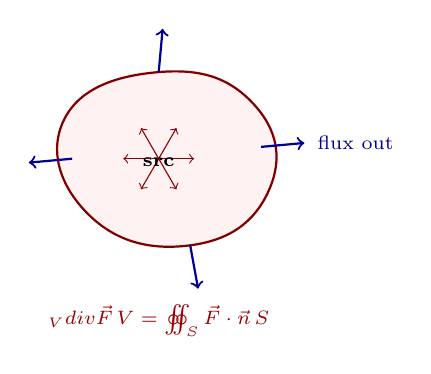
\begin{tikzpicture}[scale=1.0]
% a blob with outward normals and interior source arrows
\draw[fill=red!5,draw=red!50!black,thick] plot[smooth cycle,tension=0.8]
  coordinates {(0,1.1)(1.2,0.7)(1.4,-0.4)(0.4,-1.1)(-0.9,-0.7)(-1.2,0.5)};
% interior source arrows (divergence > 0)
\foreach \a in {0,60,...,300}{
  \draw[->,red!55!black] (0,0) -- (\a:0.45);
}
\node at (0,-0.05) {\scriptsize\textbf{src}};
% outward normals on boundary
\draw[->,blue!60!black,thick] (1.3,0.15) -- (1.85,0.2);
\draw[->,blue!60!black,thick] (0.4,-1.1) -- (0.5,-1.65);
\draw[->,blue!60!black,thick] (-1.1,0.0) -- (-1.65,-0.05);
\draw[->,blue!60!black,thick] (0,1.1) -- (0.05,1.65);
\node[blue!60!black] at (2.5,0.2) {\scriptsize flux out};
\node[red!60!black] at (0,-2.05) {\scriptsize $\iiint_V \operatorname{div}\vec F\,\dd V = \oiint_S \vec F\cdot\vec n\,\dd S$};
\end{tikzpicture}
\caption{The divergence theorem. Sources sprinkled through the interior (red) must
balance exactly against the total flux leaving through the outer skin (blue
normals). Internal flows cancel in pairs; only the boundary is left to tell the
tale.}
\label{ch35:fig-div}
\end{figure}

\begin{example}[Divergence theorem on a ball]
\label{ch35:ex-div}
Let $\vec F=(x,y,z)$ and let $V$ be the ball of radius $a$, with $S$ its sphere.

\textbf{Left side.} $\operatorname{div}\vec F = 1+1+1 = 3$, so
\[
  \iiint_V 3\,\dd V = 3\cdot \text{Vol}(V) = 3\cdot\frac{4}{3}\pi a^3 = 4\pi a^3.
\]

\textbf{Right side.} On the sphere of radius $a$ the outward normal is
$\vec n = \frac{1}{a}(x,y,z)$, so
$\vec F\cdot\vec n = \frac{1}{a}(x^2+y^2+z^2) = \frac{a^2}{a} = a$, a constant.
Then
\[
  \oiint_S \vec F\cdot\vec n\,\dd S = a\cdot \text{Area}(S) = a\cdot 4\pi a^2 = 4\pi a^3.
\]
The two agree. The uniform source density $3$ filling the ball is paid off exactly
by the outward flux through the sphere.
\end{example}

\section{Stokes' theorem: the boundary loop of a surface}
\label{ch35:stokes}

The last of the three. Green's theorem lived in the flat plane; Stokes' theorem
lifts it into 3D, letting the surface $S$ be any curved membrane in space, like a
soap film, with the line integral run around its rim $\partial S$.

\begin{theorem}[Stokes' theorem]
\label{ch35:thm-stokes}
Let $S$ be an oriented surface in space bounded by a simple closed curve
$C=\partial S$, oriented compatibly (right-hand rule). If $\vec F$ has continuous
partials, then
\[
  \oint_C \vec F\cdot\dd\vec r \;=\; \iint_S (\operatorname{curl}\vec F)\cdot\vec n\,\dd S.
\]
\end{theorem}

\begin{intuitionbox}
The total circulation you feel marching once around the rim of a membrane equals
the sum of all the little paddlewheel spins (the curl) spread across the membrane.
And here is the wonder: \emph{any} surface with the same rim gives the same answer.
A flat disk, a tall dome, a crumpled sheet -- if they share a boundary loop, the
curl-flux through each is identical, because all that matters is the rim. (Since
$\operatorname{div}(\operatorname{curl}\vec F)=0$ always, the divergence theorem
guarantees this independence: curl has no sources, so its flux depends only on the
boundary.) Green's theorem is exactly Stokes' theorem for the special case where
$S$ is a flat region lying in the plane.
\end{intuitionbox}

\begin{happeningbox}
Same mechanism a third time. Tile the membrane $S$ with tiny patches. Around each
patch run the little circulation; by Green's theorem in miniature, that little
circulation equals $(\operatorname{curl}\vec F\cdot\vec n)\times(\text{patch area})$.
Sum over all patches. The shared edges between neighboring patches are traversed in
opposite directions and \textbf{cancel}; only the outer rim $C=\partial S$ survives.
Result: rim circulation $=$ total curl-flux. It is Green's theorem stitched over a
curved surface, and the cancellation -- yet again -- is the FTC's telescoping in
disguise.
\end{happeningbox}

\begin{figure}[H]
\centering
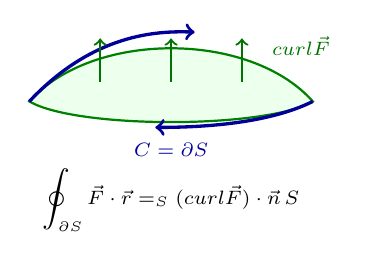
\begin{tikzpicture}[scale=1.0]
% a curved cap with boundary loop and curl arrows
\draw[fill=green!7,draw=green!50!black,thick]
  (-1.8,0) .. controls (-1,0.9) and (1,0.9) .. (1.8,0)
  .. controls (1.2,-0.35) and (-1.2,-0.35) .. (-1.8,0) -- cycle;
% boundary orientation arrows (CCW seen from above)
\draw[->,blue!60!black,very thick] (1.8,0) .. controls (1.2,-0.3) and (0.3,-0.33) .. (-0.2,-0.33);
\draw[->,blue!60!black,very thick] (-1.8,0) .. controls (-1,0.85) and (-0.2,0.9) .. (0.3,0.88);
\node[blue!60!black] at (0,-0.62) {\scriptsize $C=\partial S$};
% curl normal arrows poking up
\foreach \x in {-0.9,0,0.9}{
  \draw[->,green!45!black,thick] (\x,0.25) -- (\x,0.8);
}
\node[green!45!black] at (1.65,0.7) {\scriptsize $\operatorname{curl}\vec F$};
\node at (0,-1.25) {\scriptsize $\displaystyle\oint_{\partial S}\vec F\cdot\dd\vec r = \iint_S (\operatorname{curl}\vec F)\cdot\vec n\,\dd S$};
\end{tikzpicture}
\caption{Stokes' theorem. The circulation once around the rim $C$ (blue) equals the
flux of curl (green, poking through) across any membrane $S$ that the rim bounds.
The shape of the membrane is irrelevant; only its boundary matters.}
\label{ch35:fig-stokes}
\end{figure}

\begin{example}[Stokes on a hemisphere]
\label{ch35:ex-stokes}
Let $\vec F=(-y,x,0)$ (the swirl, lifted into 3D) and let $S$ be the upper unit
hemisphere $x^2+y^2+z^2=1$, $z\ge0$, oriented upward. Its boundary $C$ is the unit
circle in the $xy$-plane.

\textbf{Surface side.}
$\operatorname{curl}\vec F = (0,0,\,Q_x-P_y)=(0,0,1-(-1))=(0,0,2)$.
The simplest membrane with the same rim is the flat disk $z=0$, where
$\vec n=(0,0,1)$, so $(\operatorname{curl}\vec F)\cdot\vec n = 2$ and
\[
  \iint_S (\operatorname{curl}\vec F)\cdot\vec n\,\dd S = 2\cdot(\text{area of unit disk}) = 2\pi.
\]
(We are allowed to swap the hemisphere for the flat disk precisely because Stokes
says only the shared rim matters.)

\textbf{Rim side.} Parametrize $C$ by $x=\cos t$, $y=\sin t$, $z=0$:
\[
  \oint_C \vec F\cdot\dd\vec r = \int_0^{2\pi}\big[(-\sin t)(-\sin t)+(\cos t)(\cos t)\big]\dd t = 2\pi.
\]
Both give $2\pi$. The curl pointing up through the cap is precisely the swirl you
feel walking the equator.
\end{example}

\begin{historybox}
``Stokes' theorem'' was not proved by Stokes. In 1850 William Thomson (Lord Kelvin)
wrote the result in a letter to George Stokes, who then set it as a problem on the
1854 Cambridge Smith's Prize examination -- which a young James Clerk Maxwell sat.
So the theorem entered the world as an \emph{exam question}. Maxwell would later
make curl and divergence the backbone of his theory of electromagnetism. The modern
viewpoint -- that Green, Stokes, divergence, and even the plain FTC are all the
\emph{single} generalized Stokes theorem $\int_M \dd\omega = \int_{\partial M}\omega$
in the language of differential forms -- was assembled by Poincare, Cartan, and
others around 1900. One line now contains this entire chapter.
\end{historybox}

\section{One theorem, four faces}
\label{ch35:unification}

Step back and see the family resemblance. In each statement, an integral of a
\emph{derivative} over a region equals an integral of the original \emph{field}
over the region's \emph{boundary}:

\begin{center}
\renewcommand{\arraystretch}{1.6}
\begin{tabular}{@{}lll@{}}
\toprule
\textbf{Theorem} & \textbf{Inside (a derivative)} & \textbf{Boundary (the field)} \\
\midrule
FTC & $\displaystyle\int_a^b F'(x)\,\dd x$ & $F(b)-F(a)$ \\
Gradient thm & $\displaystyle\int_C \grad f\cdot\dd\vec r$ & $f(B)-f(A)$ \\
Green & $\displaystyle\iint_D (Q_x-P_y)\,\dd A$ & $\displaystyle\oint_{\partial D}\vec F\cdot\dd\vec r$ \\
Stokes & $\displaystyle\iint_S \operatorname{curl}\vec F\cdot\vec n\,\dd S$ & $\displaystyle\oint_{\partial S}\vec F\cdot\dd\vec r$ \\
Divergence & $\displaystyle\iiint_V \operatorname{div}\vec F\,\dd V$ & $\displaystyle\oiint_{\partial V}\vec F\cdot\vec n\,\dd S$ \\
\bottomrule
\end{tabular}
\end{center}

\begin{aestheticbox}
The boundary operator $\partial$ lowers dimension by one: the boundary of a solid is
a surface, of a surface a curve, of a curve two endpoints. The derivative operator
($\grad$, curl, div) is the perfect partner: applied inside, it produces exactly
what, when summed, the boundary can account for. The two are \emph{adjoint} -- that
is the one-sentence content of the generalized Stokes theorem,
$\int_M \dd\omega = \int_{\partial M}\omega$. Every theorem you have met in this
book, from $\int F' = F(b)-F(a)$ onward, is one shadow of that single sentence.
This is, to many mathematicians, the most beautiful theorem in calculus.
\end{aestheticbox}

\begin{connectionbox}
This unification is not idle elegance; it is what makes physics writable. Maxwell's
equations say $\operatorname{div}\vec E = \rho/\eps_0$ (charges are sources of the
electric field) and $\operatorname{curl}\vec B = \mu_0\vec J + \cdots$ (currents
swirl the magnetic field). Feed these into the divergence and Stokes theorems and
out come Gauss's law and Ampere's law in their boundary form -- the form you can
actually measure with a wire and a meter. The local differential law and the global
integral law are the same statement seen from inside and from the boundary.
\end{connectionbox}

\begin{labbox}
Test the unification with your hands. Take $\vec F=(-y,x)$.
(1) Compute its scalar curl. (2) Compute its divergence. (3) Use Green's theorem to
find its circulation around the boundary of the square $[0,1]\times[0,1]$, then
check it by integrating around the four edges directly. (4) Now compute its
\emph{flux} out of that same square using the flux form of Green's theorem -- and
explain, before you compute, why you expect $0$. (The swirl spins but does not
spread.)
\end{labbox}

\section{Exercises}
\label{ch35:exercises}

\begin{exercise}
\label{ch35:exr-lineint}
Compute $\displaystyle\int_C \vec F\cdot\dd\vec r$ for $\vec F=(x+y,\,y)$ along the
straight segment from $(0,0)$ to $(3,1)$. Parametrize by $\vec r(t)=(3t,t)$,
$t\in[0,1]$, and reduce to a single integral in $t$.
\end{exercise}

\begin{exercise}
\label{ch35:exr-conservative}
Show that $\vec F=(3x^2y + e^y,\; x^3 + xe^y + 2)$ is conservative by checking
$P_y=Q_x$, then find a potential $f$. Use it to evaluate $\int_C\vec F\cdot\dd\vec r$
from $(0,0)$ to $(1,1)$ along \emph{any} path.
\end{exercise}

\begin{exercise}
\label{ch35:exr-notconservative}
For $\vec F=(y,\,-x)$, compute $\oint_C\vec F\cdot\dd\vec r$ around the unit circle
counterclockwise two ways: directly by parametrization, and via Green's theorem.
Confirm they agree, and explain why the nonzero answer proves $\vec F$ is not
conservative.
\end{exercise}

\begin{exercise}
\label{ch35:exr-green-area}
Use the area formula $\text{Area}=\tfrac12\oint_C x\,\dd y - y\,\dd x$ to find the
area enclosed by the astroid $x=\cos^3 t$, $y=\sin^3 t$, $t\in[0,2\pi]$. (You should
get $\tfrac{3}{8}\pi$.)
\end{exercise}

\begin{exercise}
\label{ch35:exr-divcurl}
For $\vec F=(x^2 y,\; -xy^2,\; z)$ compute $\operatorname{div}\vec F$ and
$\operatorname{curl}\vec F$ as functions of $(x,y,z)$. Identify a point where the
field is locally incompressible ($\operatorname{div}=0$).
\end{exercise}

\begin{exercise}
\label{ch35:exr-greenverify}
Verify Green's theorem for $\vec F=(xy,\,x^2)$ over the triangle with vertices
$(0,0)$, $(1,0)$, $(1,1)$, by computing both the boundary line integral (three
edges) and the double integral of $Q_x-P_y$ over the triangle.
\end{exercise}

\begin{exercise}
\label{ch35:exr-divthm}
Use the divergence theorem to compute the flux of $\vec F=(x^3,\,y^3,\,z^3)$ out of
the unit sphere. (Hint: $\operatorname{div}\vec F = 3(x^2+y^2+z^2)$; convert the
resulting triple integral to spherical coordinates.)
\end{exercise}

\begin{exercise}
\label{ch35:exr-stokes}
Let $\vec F=(z,\,x,\,y)$ and let $S$ be the part of the paraboloid $z=1-x^2-y^2$
above the $xy$-plane, oriented upward, with boundary the unit circle. Use Stokes'
theorem to compute $\oint_{\partial S}\vec F\cdot\dd\vec r$ by integrating
$\operatorname{curl}\vec F\cdot\vec n$ over the flat unit disk instead (legal because
only the rim matters).
\end{exercise}

\begin{exercise}
\label{ch35:exr-hole}
Consider $\vec F=\big(\frac{-y}{x^2+y^2},\,\frac{x}{x^2+y^2}\big)$. (a) Verify that
its scalar curl is $0$ wherever it is defined. (b) Compute its circulation around
the unit circle and get $2\pi$. (c) Explain why parts (a) and (b) do not contradict
Green's theorem. (What goes wrong at the origin?)
\end{exercise}

\begin{exercise}
\label{ch35:exr-unify}
In your own words, state the single sentence that contains the FTC, the gradient
theorem, Green's, Stokes', and the divergence theorem at once. Identify, for each of
the five, what plays the role of ``the inside,'' ``the derivative taken inside,''
and ``the boundary.''
\end{exercise}
